\clearpage
\appendix
\section{Appendix}
We included additional bias mitigation results using other fairness metrics, such as equality of opportunity and equalized odds on both of the Adult and Heritage Health datasets in this supplementary material. We also included additional post-processing results along with additional qualitative results both for the tabular and non-tabular dataset experiments. More details can be found under each sub-section.
\subsection{Results on Tabular Data}
Here, we show the results of our mitigation framework considering equality of opportunity and equalized odds notions of fairness. We included baselines that were applicable for these notions. Notice not all the baselines we used in our previous analysis for statistical parity were applicable for equality of opportunity and equalized odds notions of fairness; thus, we only included the applicable ones. In addition, LAFTR is only applicable when the sensitive attribute is a binary variable, so it was not applicable to be included in the analysis for the heritage health data where the sensitive attribute is non-binary. Results of these analysis is shown in Figures~\ref{mitig_results_eqop} and \ref{mitig_results_eqod}. We once again show competitive and comparable results to other baseline methods, while having the advantage of being interpretable and not requiring multiple trainings to satisfy different fairness notions or fairness on different sensitive attributes. Our framework is also flexible for different fairness measures and can be applied to binary or non-binary sensitive features.


In addition, we show how different features contribute differently under different fairness notions. Fig.~\ref{features} demonstrates the top three features that contribute to unfairness the most along with the percentages of the fairness improvement upon their removal for each of the fairness notions. As observed from the results, while equality of opportunity and equalized odds are similar in terms of their problematic features, statistical parity has different trends. This is also expected as equality of opportunity and equalized odds are similar fairness notions in nature compared to statistical parity.

We also compared our mitigation strategy with the Hardt etl al. post-processing approach~\cite{NIPS2016_9d268236}. Using this post-processing implementation~\footnote{\url{https://fairlearn.org}}, we obtained the optimal solution that tries to satisfy different fairness notions subject to accuracy constraints. For our results, we put the results from zeroing out all the attention weights corresponding to the problematic features that were detected from our interpretability framework. However, notice that since our mitigation strategy can control different trade-offs we can have different results depending on the scenario. Here, we reported the results from zeroing out the problematic attention weights that is targeting fairness mostly. From the results demonstrated in Tables~\ref{adult_post_proc} and~\ref{health_post_proc}, we can see comparable numbers to those obtained from~\cite{NIPS2016_9d268236}. This again shows that our interpretability framework yet again captures the correct responsible features and that the mitigation strategy works as expected.

\subsection{Results on non-tabular Data}
We also included some additional qualitative results from the experiments on non-tabular data in Fig.~\ref{fig:NLP_qualitative_appendix}.
\begin{figure*}[h]
    \centering
      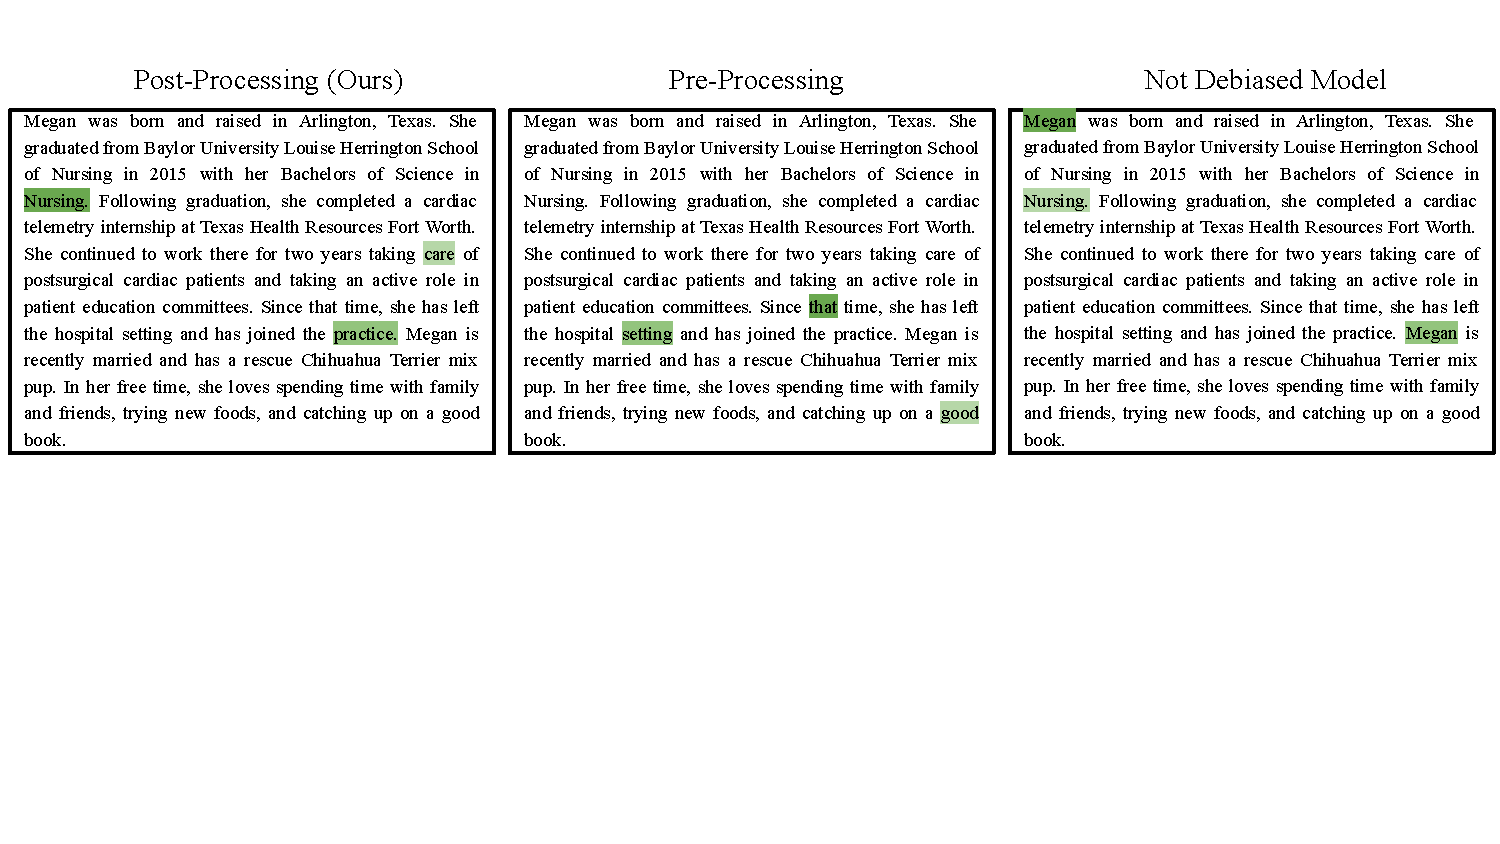
\includegraphics[width=\textwidth,trim=0cm 6cm 0cm 1cm,clip=true]{./images/NLP_qual/ex3.pdf}
    \caption{Additional qualitative results from the non-tabular data experiment on the job classification task based on the bio texts. Green regions represent top three words that the model used for its prediction based on the attention weights.}
    \label{fig:NLP_qualitative_appendix}
\end{figure*}

\subsection{Interpreting Fairness with Attention}
Fig.~\ref{fig:interpret_results_2} shows results on a subset of the features from the \textit{UCI Adult} and \textit{Heritage Health} datasets (to keep the plots uncluttered and readable, we incorporated the most interesting features in the plot), and  provide some intuition about how different features in these datasets contribute to the model fairness and accuracy. While features such as {\em capital gain} and {\em capital loss} in the \textit{UCI Adult} dataset are responsible for improving accuracy and reducing bias, we can observe  that features such as {\em relationship} or {\em marital status}, which can be indirectly correlated with the feature {\em sex}, have a negative impact on fairness. For the \textit{Heritage Health} dataset, including the features {\em drugCount ave} and {\em dsfs max} provide accuracy gains but at the expense of fairness, while including {\em no Claims} and {\em no Specialities} negatively impact both accuracy and fairness. 


\subsection{Information on Datasets and Features}
More details about each of the datasets along with the descriptions of each feature for the Adult dataset can be found at\footnote{https://archive.ics.uci.edu/ml/datasets/adult} and for the Heritage Health dataset can be found at
\footnote{https://www.kaggle.com/c/hhp}. In our qualitative results, we used the feature names as marked in these datasets. If the names or acronyms are unclear kindly reference to the references mentioned for more detailed description for each of the features. Although most of the features in the Adult datasets are self-descriptive, Heritage Health dataset includes some abbreviations that we list in Table~\ref{feature_abbriv} for the ease of interpreting each feature's meaning.

\begin{table}[h]
\centering
\begin{tabular}{|c|c|}
\hline
\textbf{Abbreviation}                     & \textbf{Meaning}                                                         \\ \hline
\multirow{1}{*}{PlaceSvcs}      & Place where the member was treated.         
                                                          \\ \hline
\multirow{1}{*}{LOS}   & Length of stay.                  
                              \\ \hline
\multirow{1}{*}{dsfs} & Days since first service that year.            
                                           \\ \hline
\end{tabular}
\caption{Some abbreviations used in Heritage Health dataset's feature names. These abbreviations are listed for clarity of interpreting each feature's meaning specifically in our qualitative analysis or attribution visualizations.}
\label{feature_abbriv}
\end{table}

\begin{figure*}[h]
\begin{subfigure}[b]{0.49\textwidth}
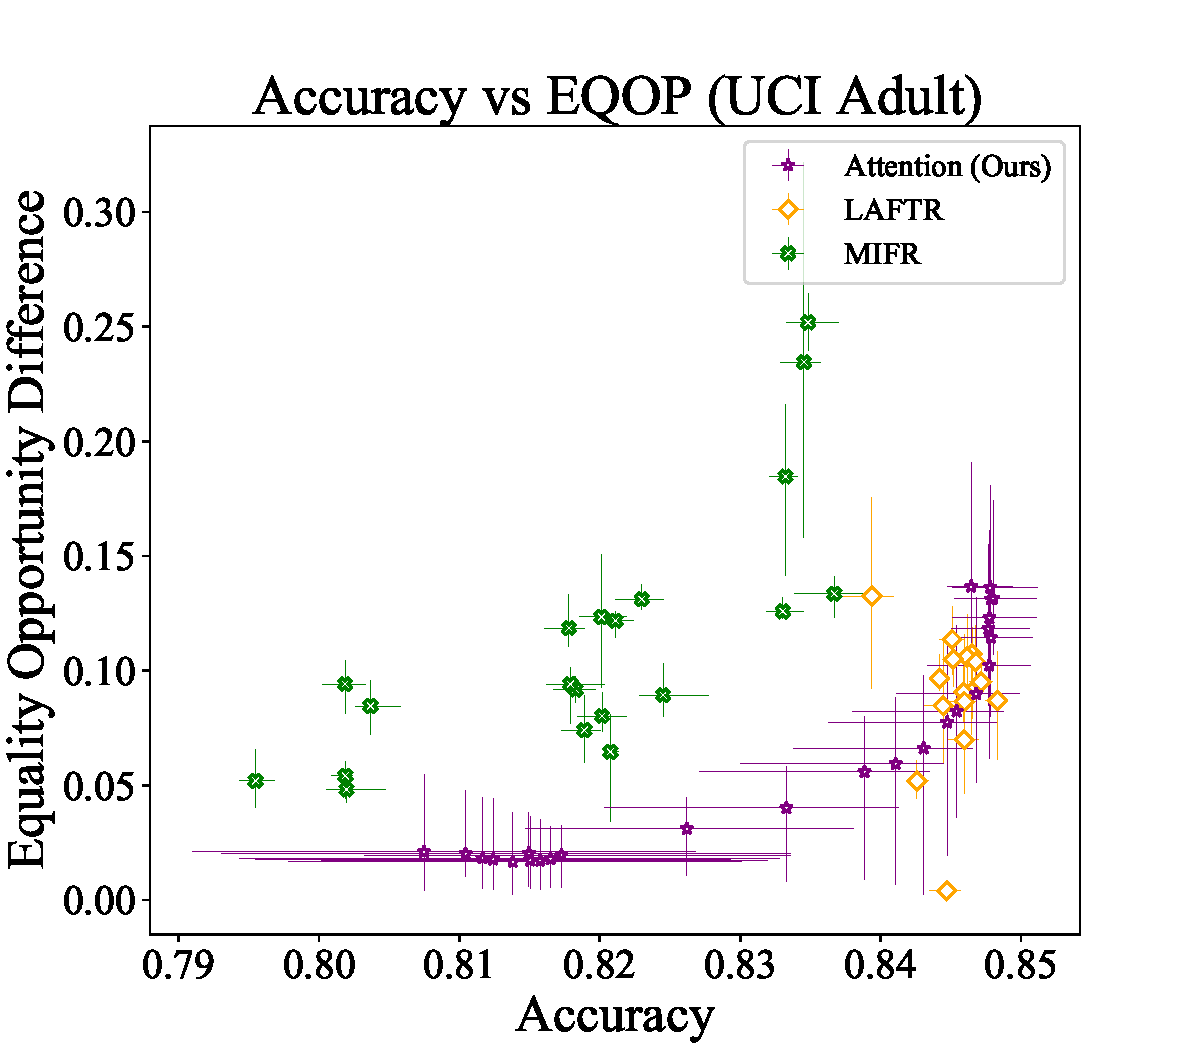
\includegraphics[width=\textwidth,trim=0cm 0cm 1.8cm 1.0cm,clip=true]{./images/appendix_imgs/adult_results_err_eqop.pdf}
\end{subfigure}
\begin{subfigure}[b]{0.49\textwidth}
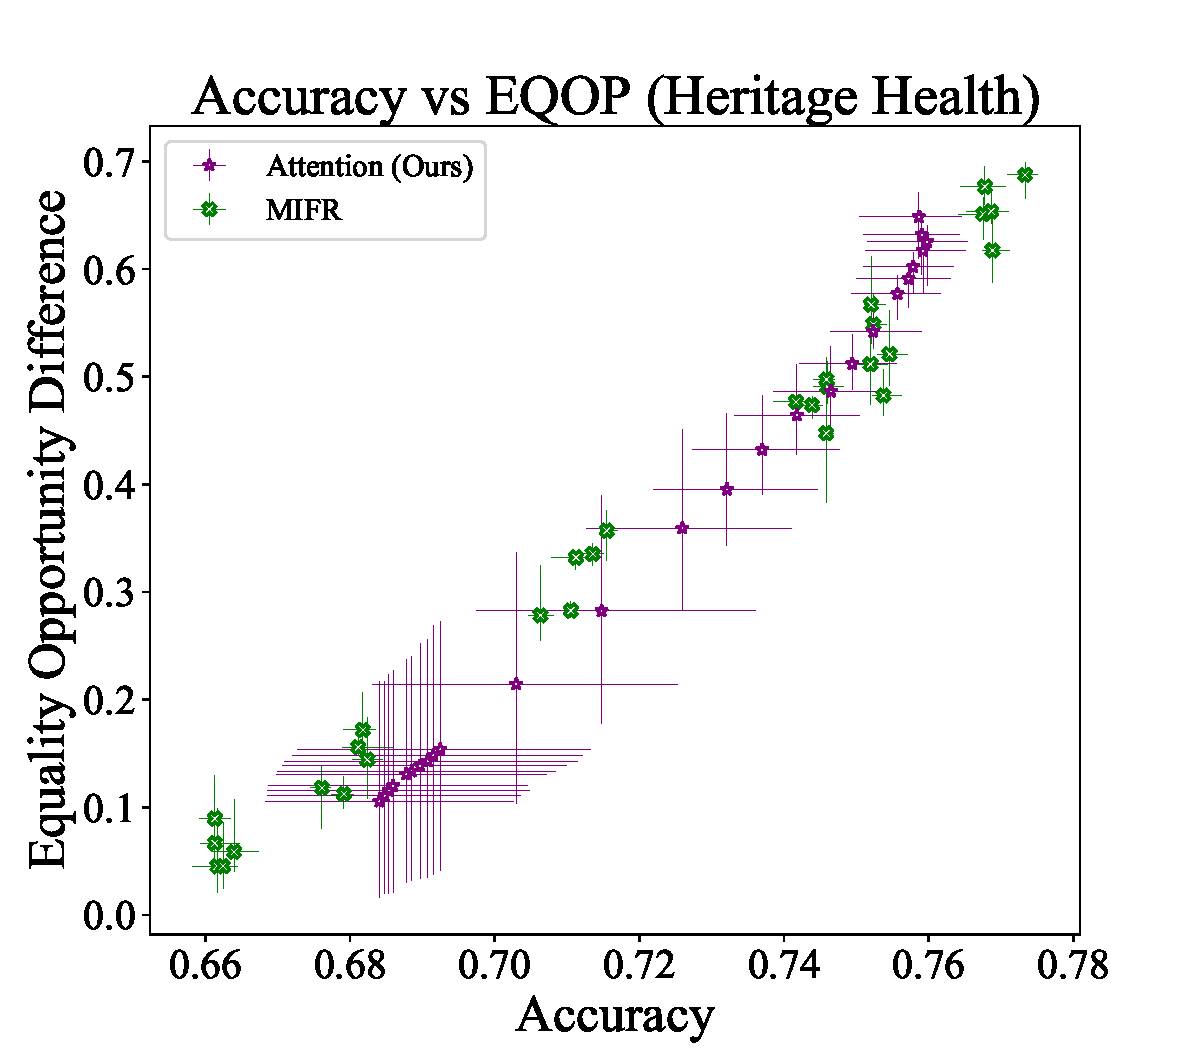
\includegraphics[width=\textwidth,trim=0cm 0cm 1.8cm 1cm,clip=true]{./images/appendix_imgs/health_results_err_eqop.pdf}
\end{subfigure}
\caption{Accuracy vs equality of opportunity curves for UCI Adult and Heritage Health datasets.}
\label{mitig_results_eqop}
\end{figure*}


\begin{figure*}[h]
\begin{subfigure}[b]{0.49\textwidth}
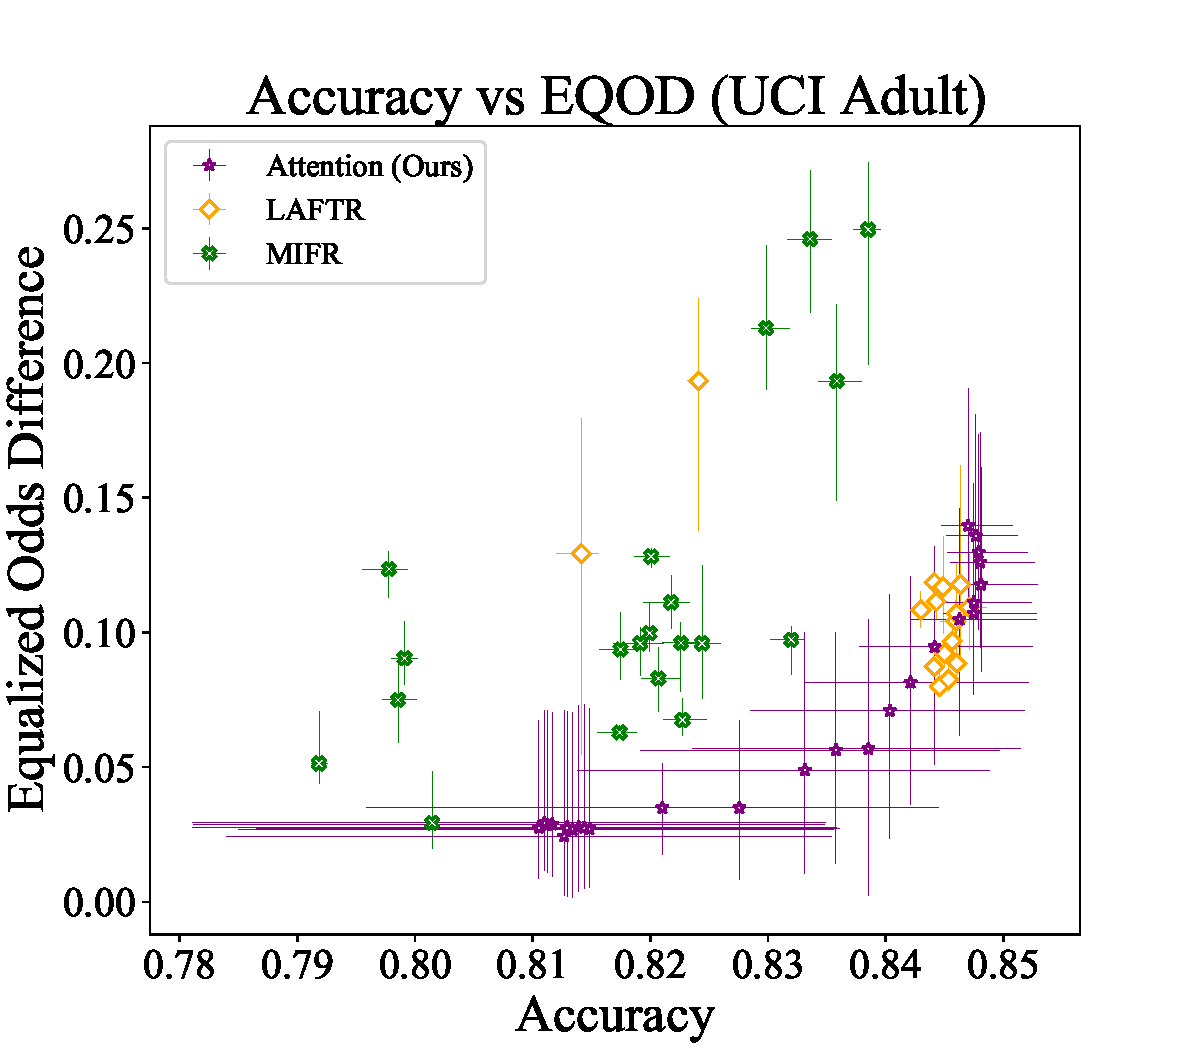
\includegraphics[width=\textwidth,trim=0cm 0cm 1.8cm 1.0cm,clip=true]{./images/appendix_imgs/adult_results_err_eqod.pdf}
\end{subfigure}
\begin{subfigure}[b]{0.49\textwidth}
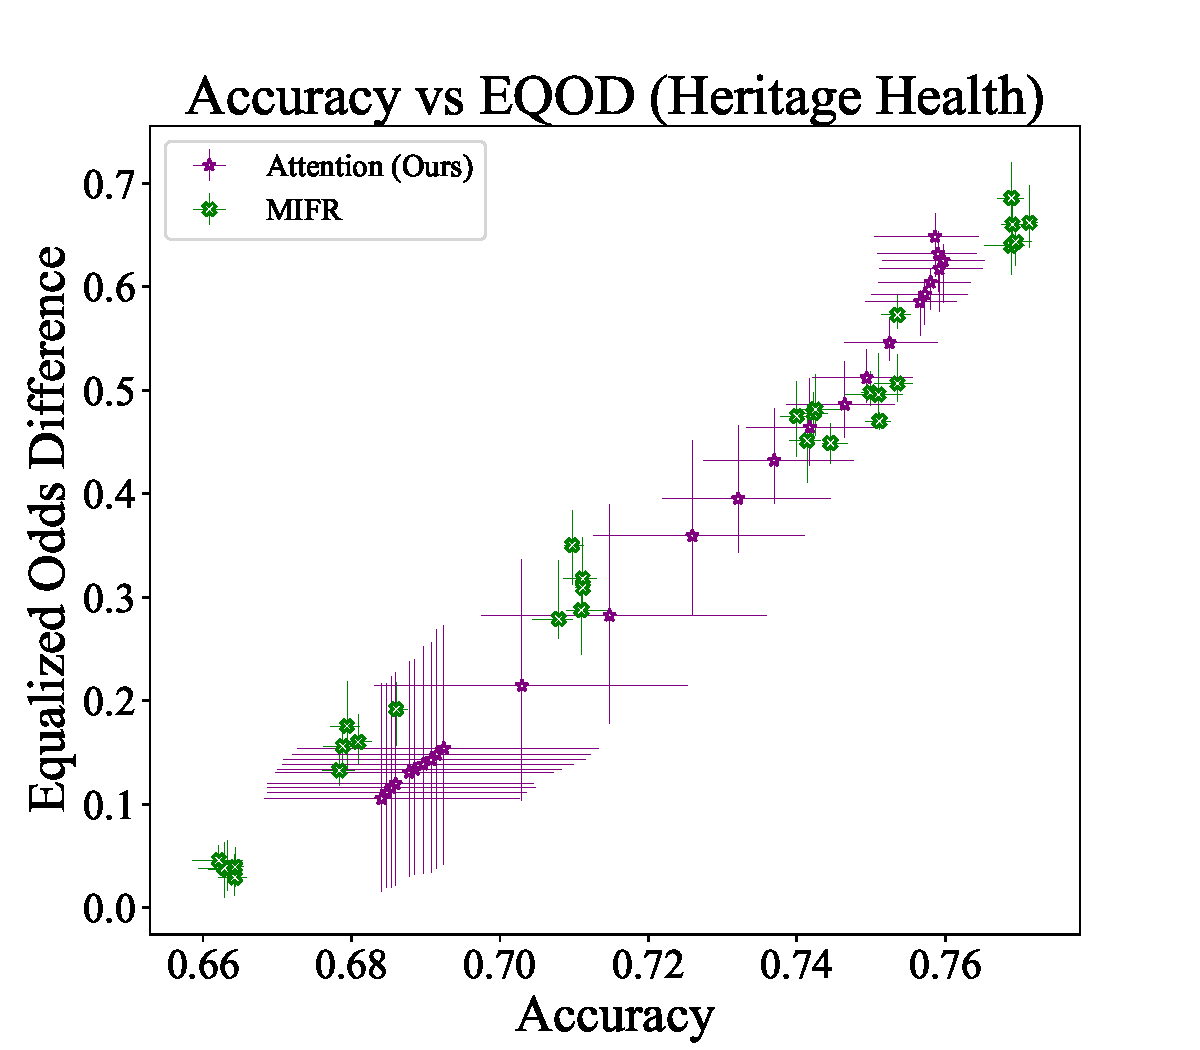
\includegraphics[width=\textwidth,trim=0cm 0cm 1.8cm 1cm,clip=true]{./images/appendix_imgs/health_results_err_eqod.pdf}
\end{subfigure}
\caption{Accuracy vs equalized odds curves for UCI Adult and Heritage Health datasets.}
\label{mitig_results_eqod}
\end{figure*}

\begin{figure*}[h]
\centering
\begin{subfigure}[b]{0.44\textwidth}
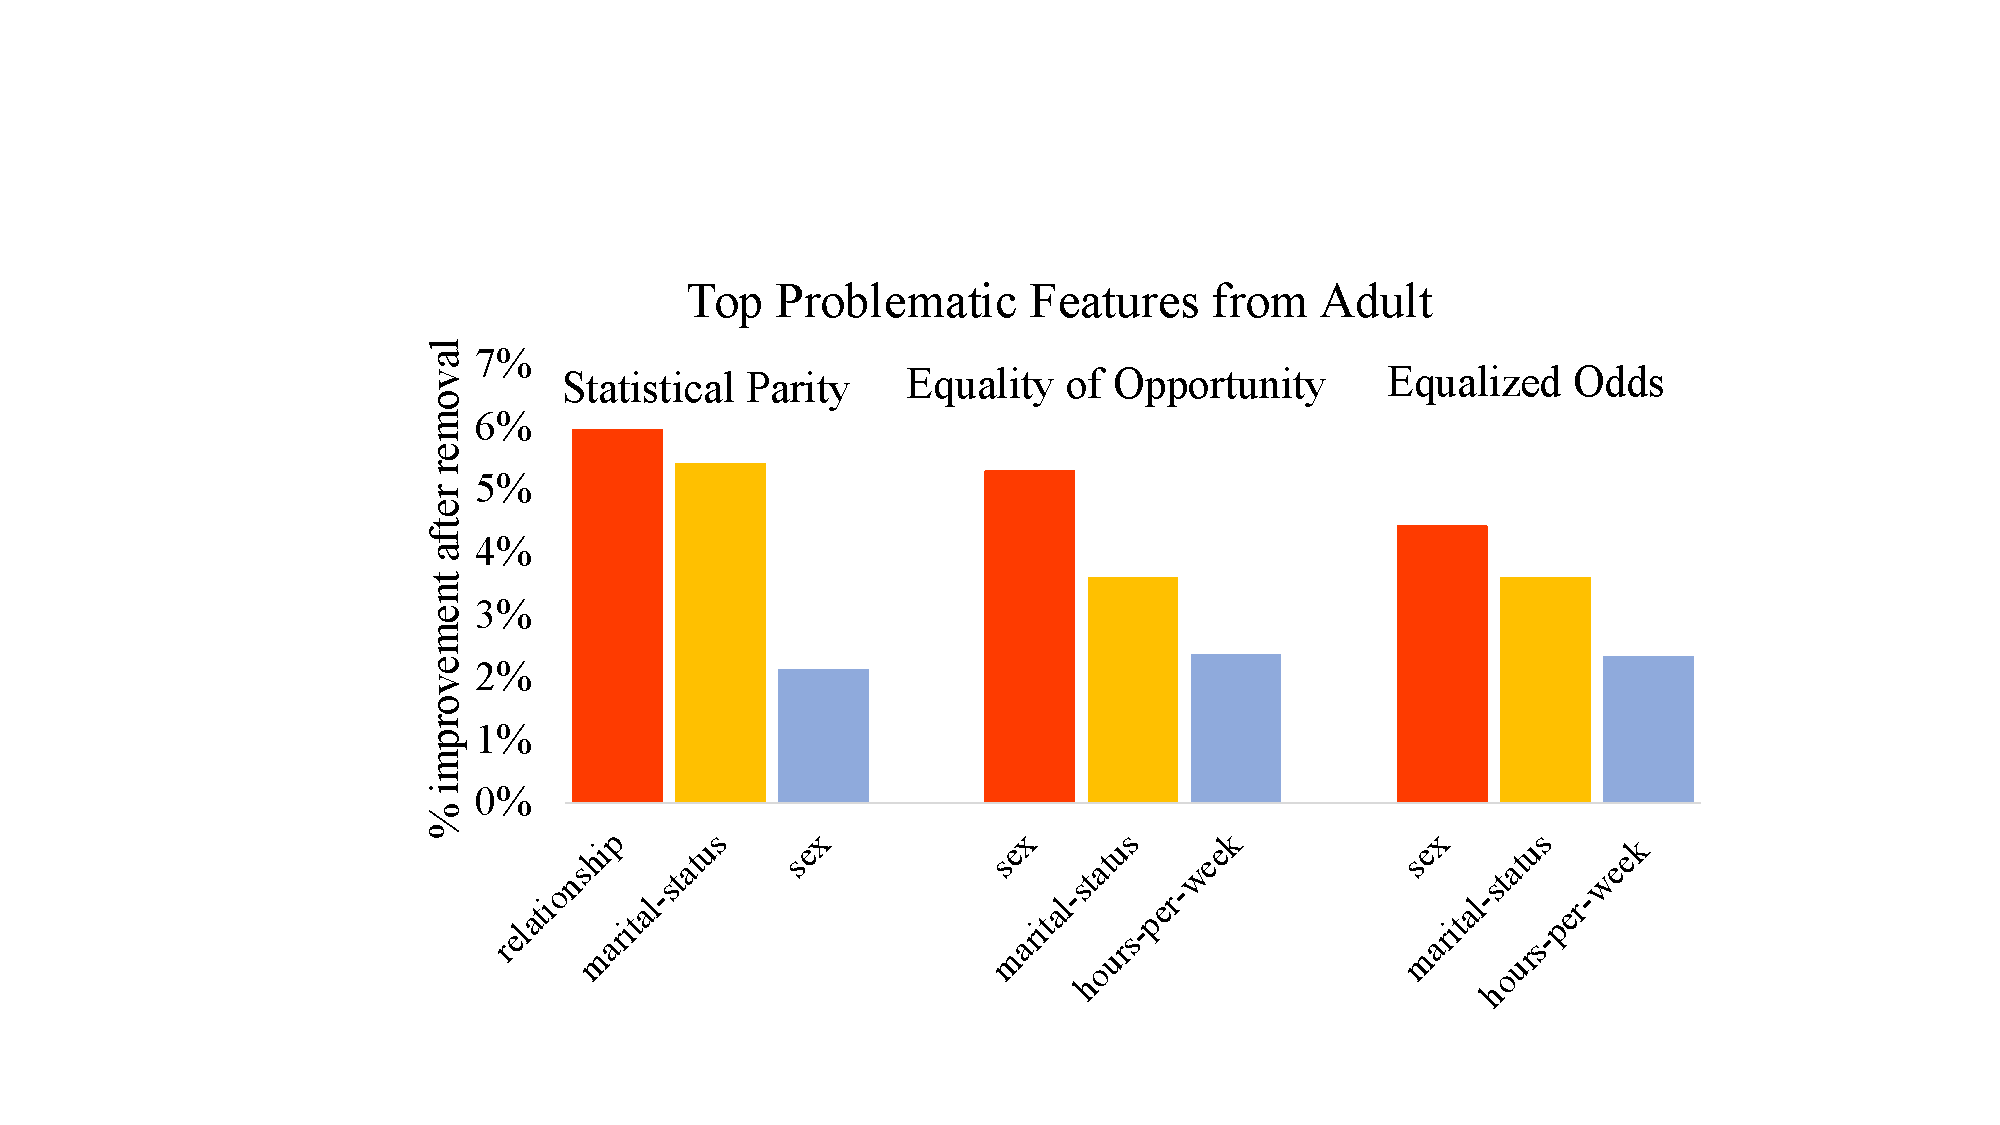
\includegraphics[width=\textwidth,trim=7cm 2cm 5cm 4cm,clip=true]{./images/appendix_imgs/adult_features.pdf}
\end{subfigure}
\begin{subfigure}[b]{0.50\textwidth}
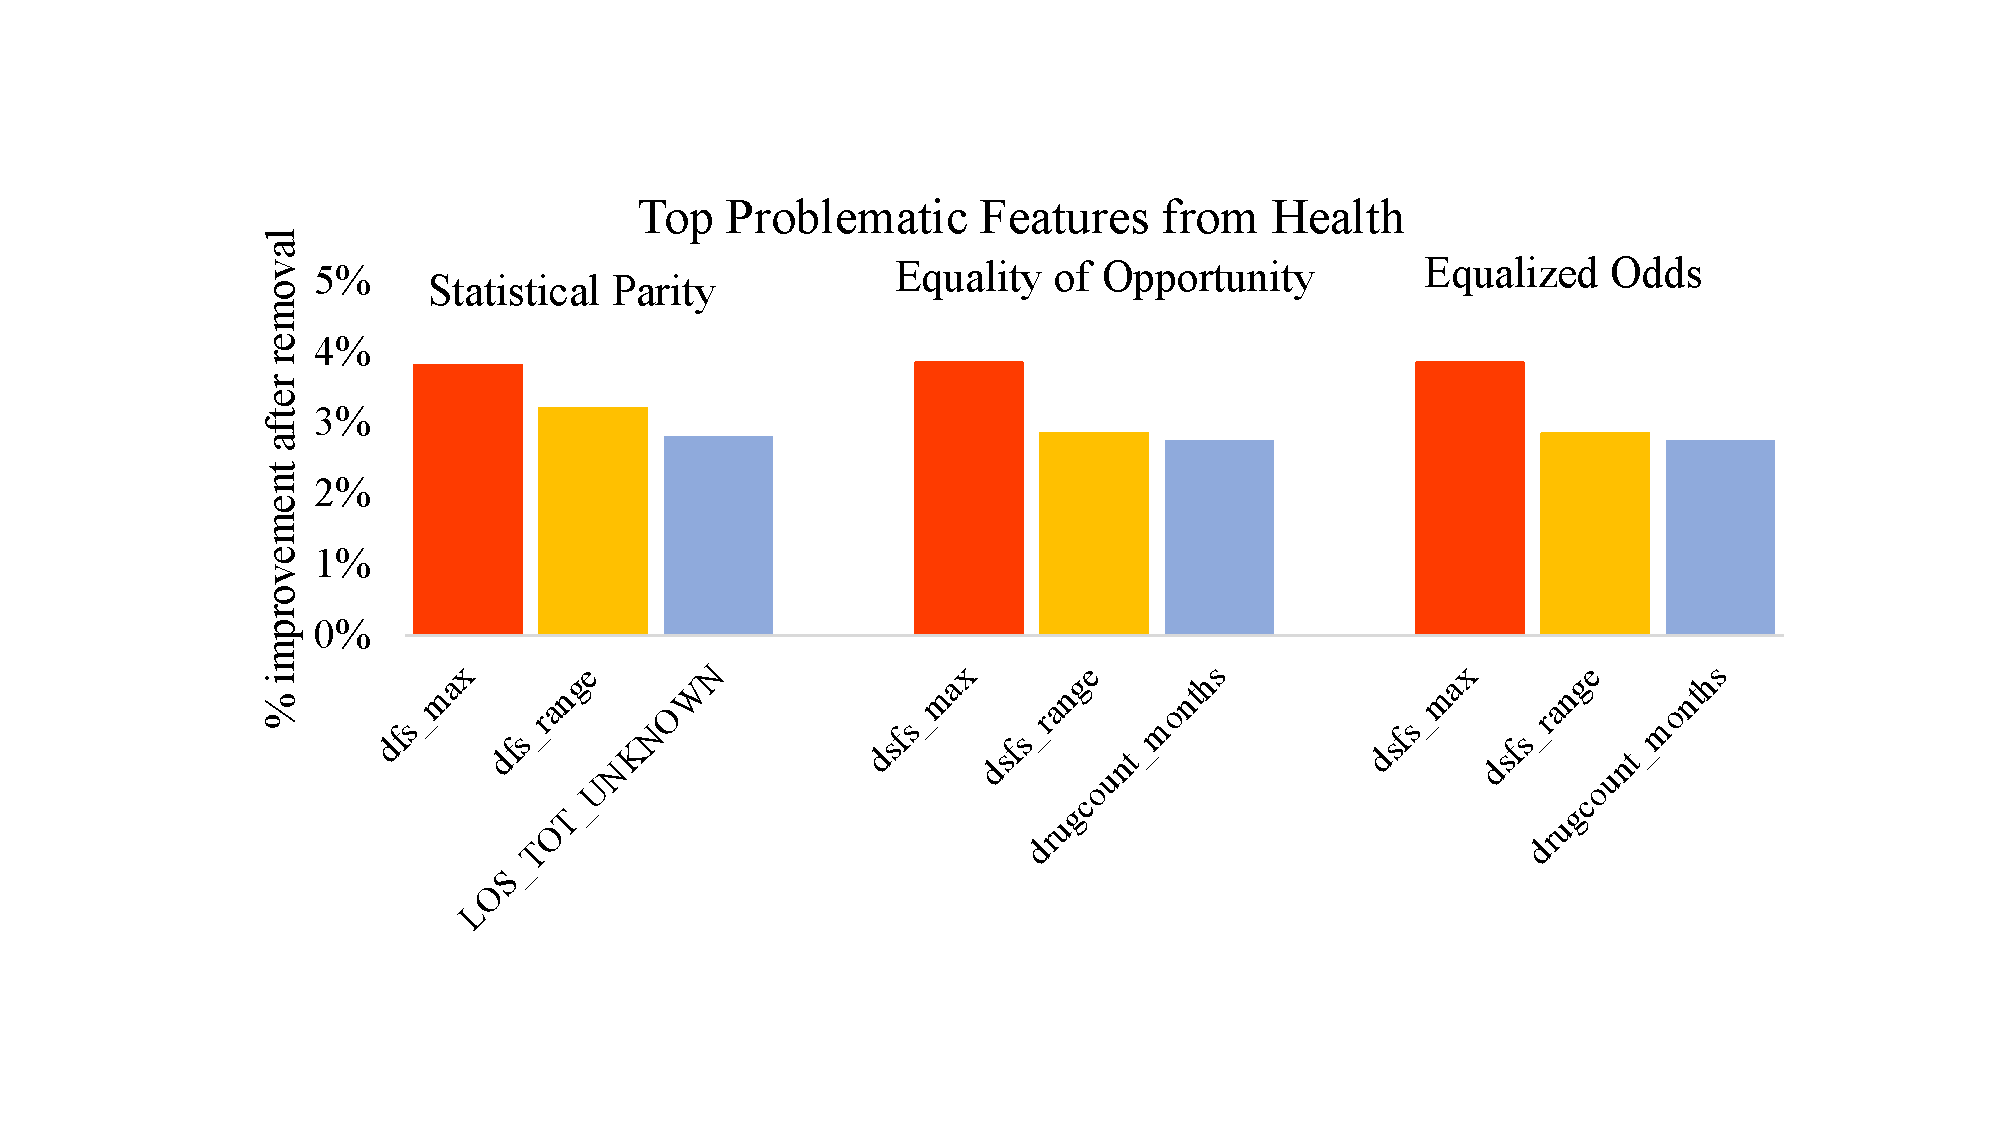
\includegraphics[width=\textwidth,trim=4cm 3cm 4cm 3cm,clip=true]{./images/appendix_imgs/health_features.pdf}
\end{subfigure}
\caption{Top three features for each fairness definition removing which caused the most benefit in improving the corresponding fairness definition. The percentage of improvement upon removal is marked on the $y$-axis for adult and heritage health datasets.}
\label{features}
\end{figure*}

\begin{table*}[h]
\centering
\scalebox{0.9}{
    \begin{tabular}{c | c c  | c c |cc}
        \toprule
        & Accuracy & SPD   & Accuracy & EQOP & Accuracy & EQOD\\
        \midrule
        Attention (Ours)&\textbf{0.77 (0.006)}&\textbf{0.012 (0.003)}&0.81 (0.013)&\textbf{0.020 (0.019)}&\textbf{0.81 (0.021)}&\textbf{0.027 (0.023)}\\
        \midrule
        Hardt et al.&\textbf{0.77 (0.012)}&0.013 (0.005)&\textbf{0.83 (0.005)}&0.064 (0.016)&\textbf{0.81 (0.007)}&0.047 (0.014)\\
        \bottomrule
    \end{tabular}}
    \caption{Adult results on post-processing approach from Hardt et al. vs our attention method when all problematic features are zeroed out.}
    \label{adult_post_proc}
    \vspace{-1em}
\end{table*}


\begin{table*}[h]
\centering
\scalebox{0.9}{
    \begin{tabular}{c | c c  | c c |cc}
        \toprule
        & Accuracy & SPD  & Accuracy & EQOP & Accuracy & EQOD\\
        \midrule
        Attention (Ours)&\textbf{0.68 (0.004)}&\textbf{0.04 (0.015)}&0.68 (0.015)&\textbf{0.15 (0.085)}&0.68 (0.015)&\textbf{0.10 (0.085)}\\
        \midrule
        Hardt et al.&\textbf{0.68 (0.005)}&0.05 (0.018)&\textbf{0.75 (0.001)}&0.20 (0.033)&\textbf{0.69 (0.012)}&0.19 (0.031)\\
        \bottomrule
    \end{tabular}
    }
    \caption{Heritage Health results on post-processing approach from Hardt et al. vs our attention method when all problematic features are zeroed out.}
    \label{health_post_proc}
    \vspace{-1em}
\end{table*}

\begin{figure*}[h]
\centering
\begin{subfigure}[b]{0.45\textwidth}
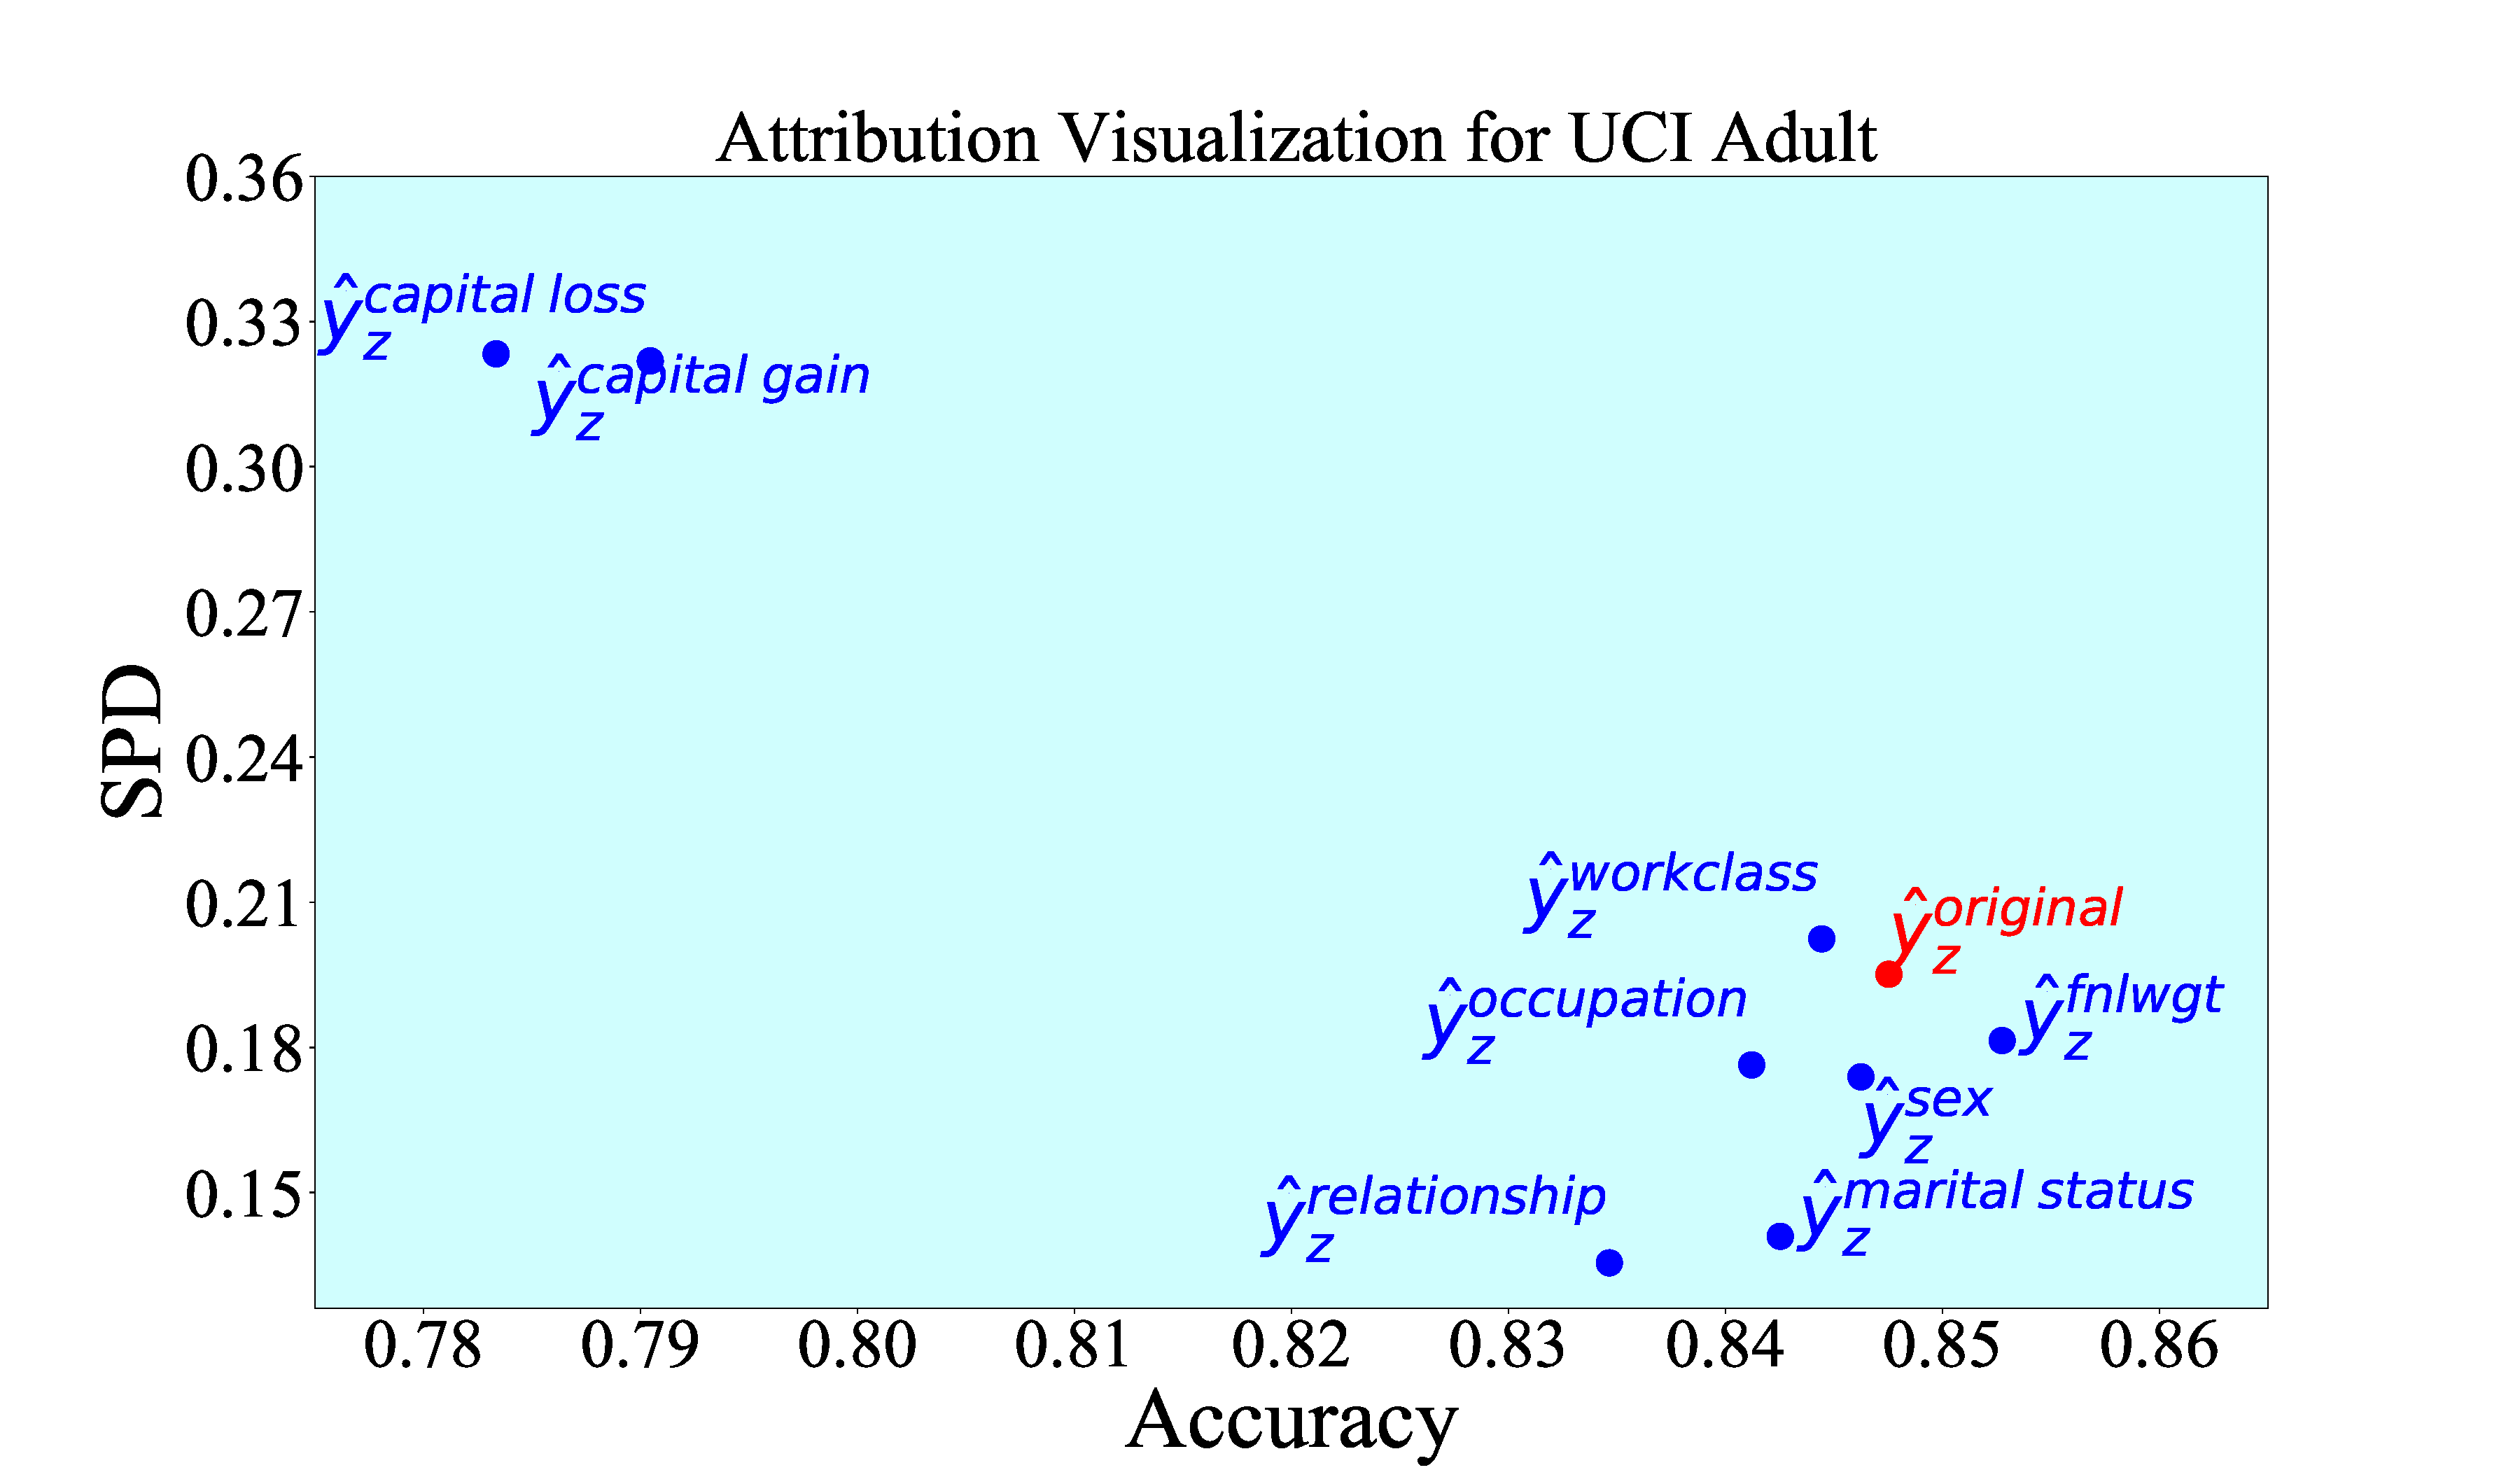
\includegraphics[width=\textwidth,trim=2.5cm 0cm 4.5cm 1.0cm,clip=true]{./images/inter_imgs/attr_vis_adult.pdf}
\end{subfigure}
\begin{subfigure}[b]{0.45\textwidth}
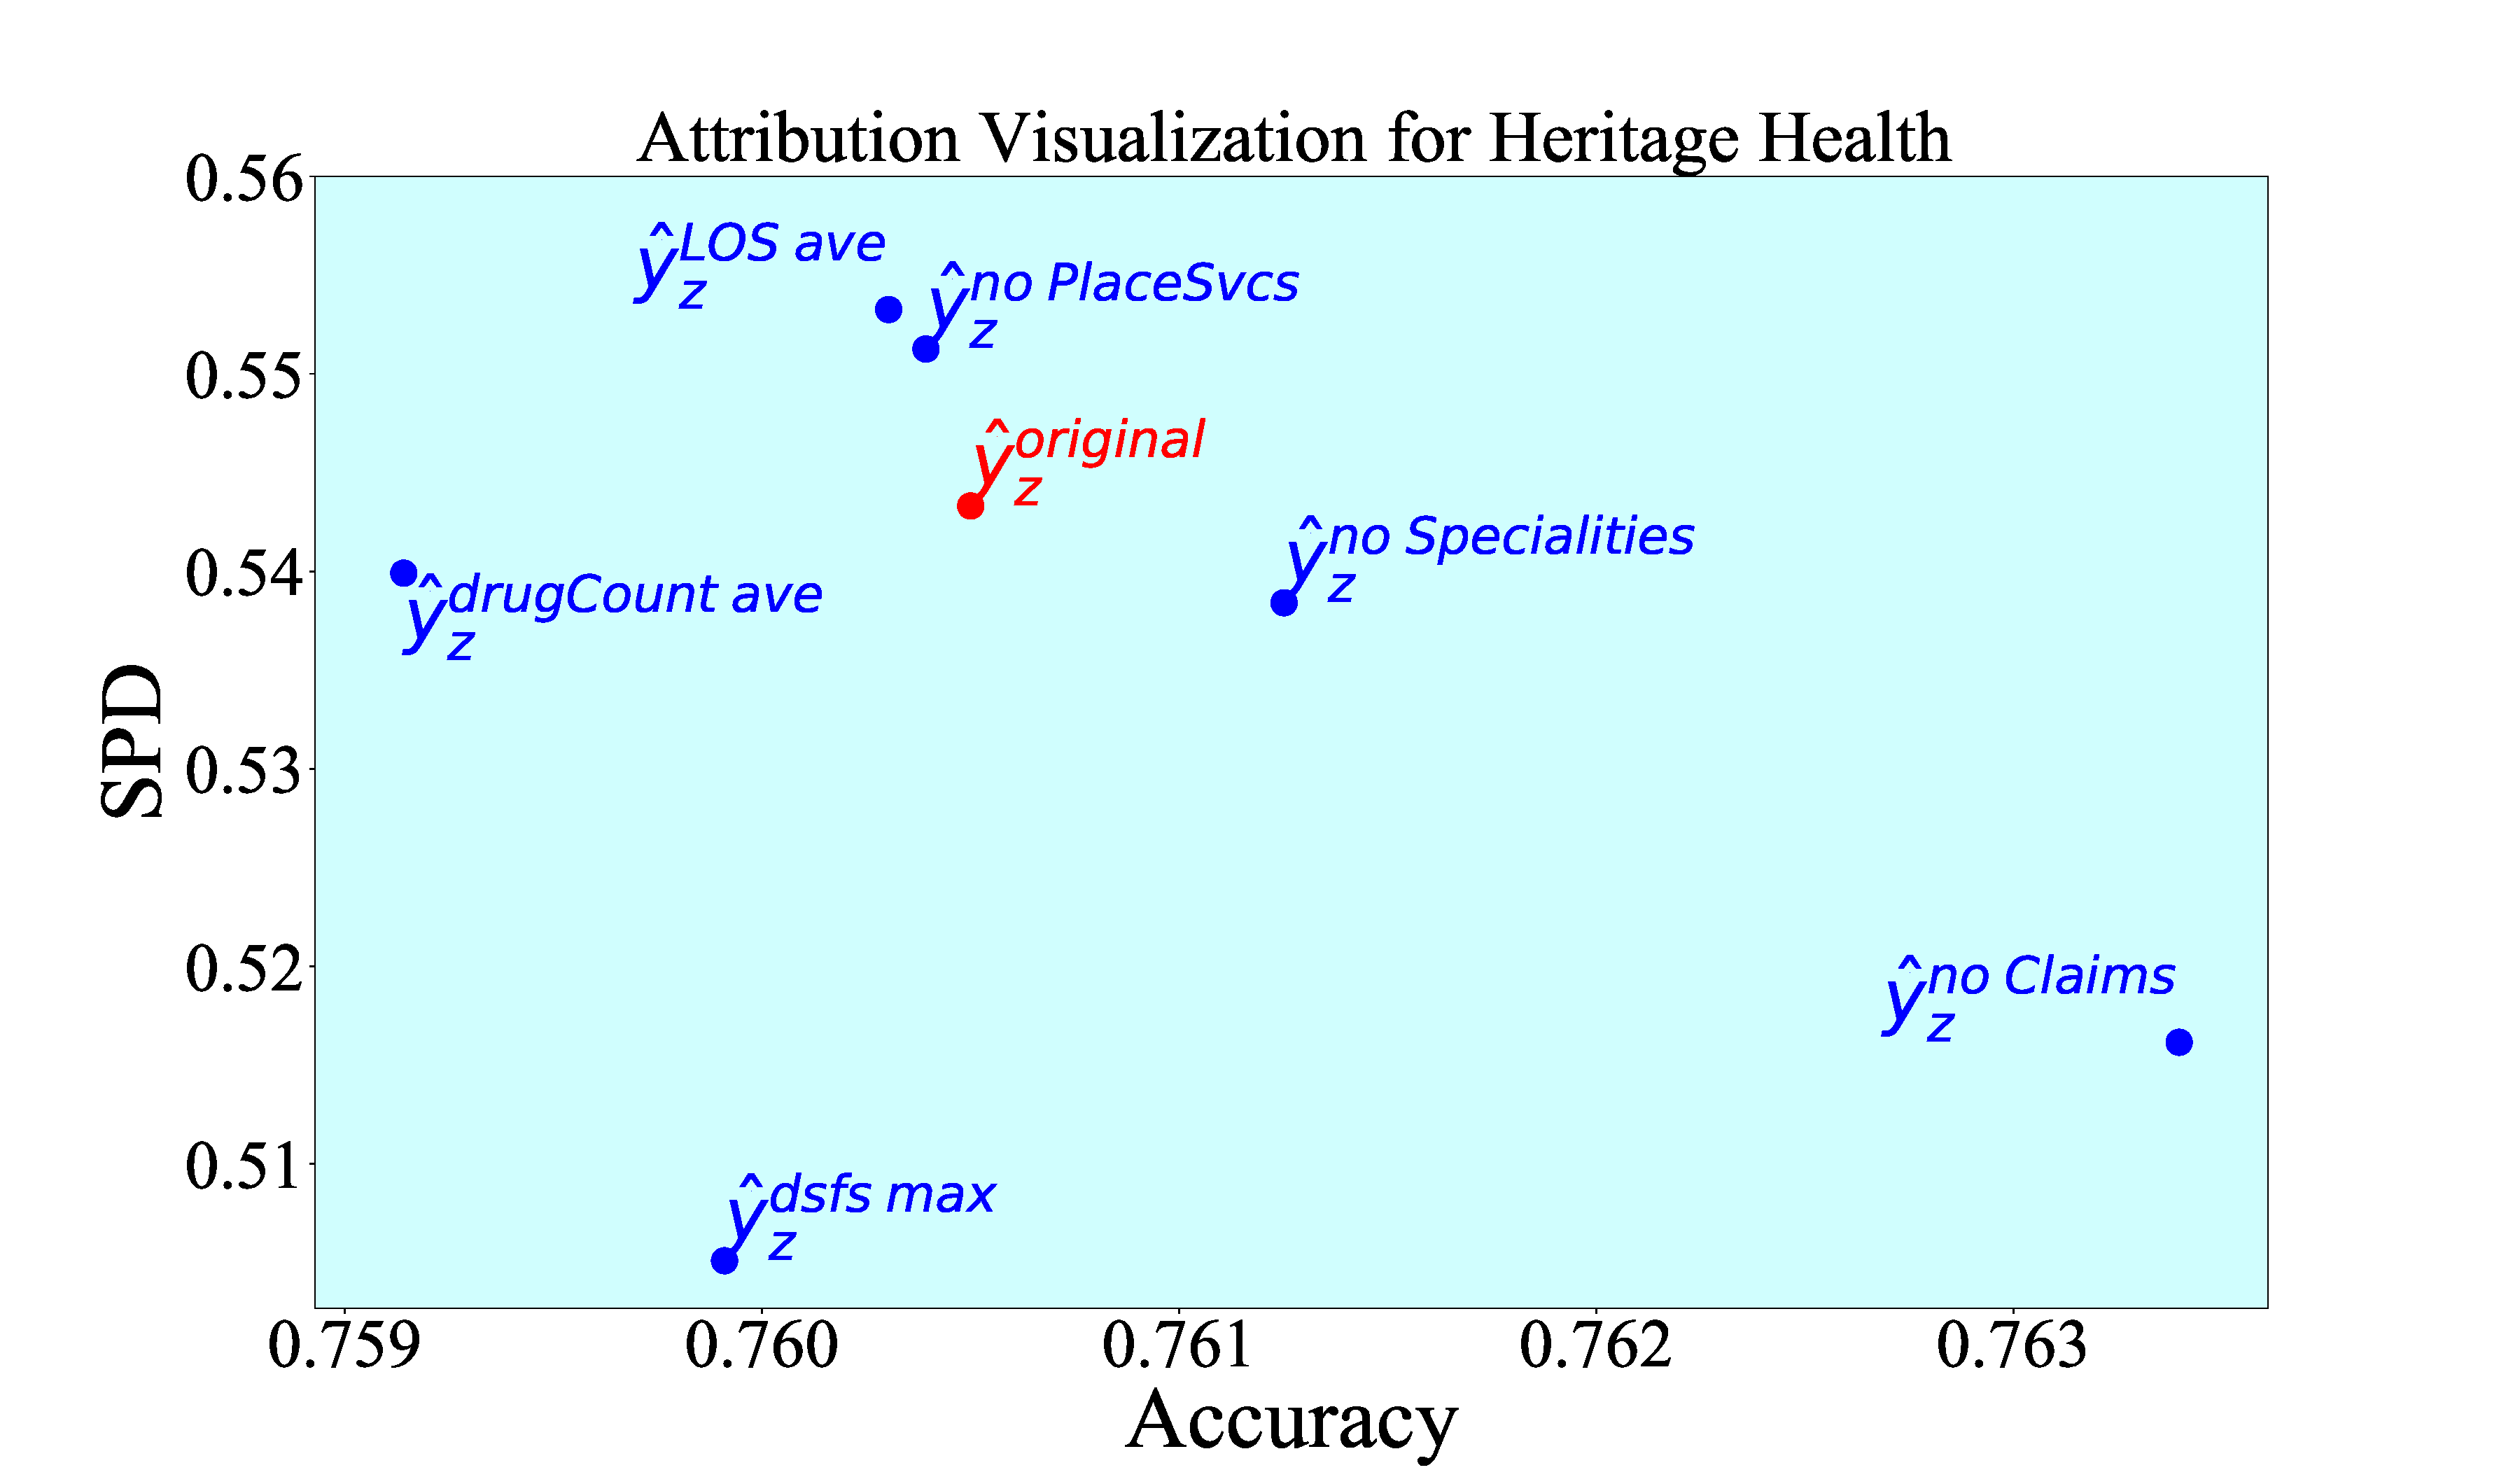
\includegraphics[width=\textwidth,trim=2.4cm 0cm 4.5cm 1.0cm,clip=true]{./images/inter_imgs/attr_vis_health.pdf}
\end{subfigure}
\caption{Results from the real-world datasets. Note that in our $\hat{y}_z$ notation we replaced indexes with actual feature names for clarity in these results on real-world datasets as there is not one universal indexing schema, but the feature names are more universal and discriptive for this case. Labels on the points represent the feature name that was removed (zeroed out) according to our $\hat{y}_z$ notation. The results show how the accuracy and fairness of the model (in terms of statistical parity difference) change by exclusion of each feature.}
\label{fig:interpret_results_2}
\end{figure*}